\chapter{\IfLanguageName{dutch}{Methodologie}{Methodology}}
\label{ch:methodologie}

In dit hoofdstuk werden alle tools uit hoofdstuk ~\ref{lab:tools} vergeleken met elkaar om zo een best passende tool voor het onderzoek te vinden. Aan de hand van een ''MoSCoW''-analyse werd bepaald wat de vereisten waren. Een deel van de vereisten zijn bepaald aan de hand van voorgaand onderzoek \autocite{Cedric2019}. Het andere deel werd bepaald aan de hand van de bachelorproef opdracht en communicatie met de (co)promotor.
 
\begin{itemize}
    \item Must have: alle noodzakelijke eigenschappen
    \item Should have: eigenschappen die niet verplicht zijn, maar wel een meerwaarde zijn
    \item Could have: eigenschappen die een kleine meerwaarde hebben
    \item Would have: alles wat een meerwaarde kan hebben maar niet nodig is voor dit onderzoek
\end{itemize}

Tenslotte werd de opstelling van het onderzoek uitgelegd. Aan de hand van die opstelling werd een checklist opgemaakt en in de conclusie een antwoord geformuleerd op de onderzoeksvraag.\clearpage

\section{Requirements-analyse}
\subsection{Must have}
\begin{itemize}
    \item De tool moet gratis zijn of de trial moet lang genoeg duren.
    \item De tool moet voor een containeromgeving zijn.
    \item De volledige PoC moet lokaal geïnstalleerd zijn.
    \item De PoC moet mogelijk zijn op de laptop van de studenten die voldoet aan de opgelegde specificaties van HoGent.
    \item Via de Proof-Of-Concept moeten de functies van de monitoringtool goed genoeg zijn om de I/O metrics te analyseren.
\end{itemize}

\subsection{Should have}

\begin{itemize}
    \item Aan de hand van één bestand kan de Proof-of-Concept opgezet worden zodat de studenten direct aan de slag kunnen met de monitoringtool.
    \item Installatie en configuratie moet van een gemiddeld niveau zijn.
\end{itemize}

\subsection{Could have}

\begin{itemize}
    \item Opzetten van alerts.
\end{itemize}

\subsection{Would have}

\begin{itemize}
    \item Het verzamelen en analyseren van logs. 
\end{itemize}
\clearpage
\section{Onderzoeksmethodologie}

Eerder vermeld in dit onderzoek, luidt de volgende onderzoeksvraag:

\begin{itemize}
    \item Welke monitoringtool voor een Kubernetes/Docker environment is het meest geschikt voor de studenten toegepaste informatica om zo een goede basiskennis te bekomen.
\end{itemize}

Eveneens zijn er nog een aantal deelvragen die ook belangrijk zijn:

\begin{itemize}
    \item Wat zijn de belangrijkste verschillen tussen de tools?
    \item Waar moeten de tools inzicht op geven?
    \item Welk proof-of-concept is voldoende om de tool aan te leren?
\end{itemize}

Om een antwoord te formuleren op de vragen wordt een onderzoek gevoerd in verschillende stappen.

\begin{itemize}
    \item Stap 1: Vergelijken van de tools op basis van de requirements-analyse.
    \item Stap 2: Opstellen van een Proof-of-Concept.
    \item Stap 3: Checklist overlopen met de vereisten.
\end{itemize}

\section{Stap 1: Vergelijken van de tools}
 
Aan de hand van een aantal vooropgestelde vereisten werden de tools vergeleken en zo werd beslist welke tool de beste was voor de PoC. Het eerste deel van de vergelijking werd gedaan aan de hand van de vereisten die opgesteld waren in de ''must have'' sectie van de MoSCoW-strategie. Tenslotte werden de tools ook vergeleken met de andere secties van de strategie.

\subsection{Vergelijking op basis van de must haves}

Zoals de naam al aangeeft, bestaat deze sectie uit initiatieven die een ''must'' zijn. Indien een tool niet aan de verwachtingen voldeed die in de analyse aangegeven waren, was de tool niet geschikt voor de Proof-of-Concept en werd deze in het verloop van de analyse niet verder onderzocht.

De volgende vereisten werden voordien opgesteld:

\begin{itemize}
    \item De tool moet gratis zijn of de trial moet lang genoeg duren.
    \item De tool moet voor een containeromgeving zijn.
    \item De volledige PoC moet lokaal geïnstalleerd zijn.
    \item De PoC moet mogelijk zijn op de laptop van de studenten die voldoet aan de opgelegde specificaties van HoGent.
    \item Via de Proof-Of-Concept moeten de functies van de monitoringtool goed genoeg zijn om de I/O metrics te analyseren.
\end{itemize}

\clearpage

\subsubsection{De tool moet gratis zijn of de trial moet lang genoeg duren}

Deze ''must have'' werd eerst bekeken omdat de grootste splitsing hier zou gebeuren. De tool moest gratis zijn of de trial moest lang genoeg duren en 30 dagen was hiervoor voldoende. Op Scout en Pingdom na waren alle tools gratis. Doordat Pingdom een trial beschikbaar stelde die lang genoeg duurde, werd deze ook opgenomen naar de volgende vereiste. Scout had ook een trial maar deze duurde maar 14 dagen. 

\subsubsection{De tool moet voor een containeromgeving zijn}

In theorie kan elke tool die lokaal op Linux draait, ook in een containeromgeving worden opgesteld. Maar voor deze ''must have'' werd gekeken naar tools die ontwikkeld zijn voor een containeromgeving. Uit onderzoek is gebleken dat alle tools geschikt waren voor een containeromgeving. Hoewel Datadog een cloud tool was, was deze toch bruikbaar voor een containeromgeving door het gebruik van een agent. Sensu's componenten waren niet dockerized maar waren toch bruikbaar in een containeromgeving.

\subsubsection{De volledige PoC moet lokaal geïnstalleerd zijn}

De volledige PoC moest lokaal geïnstalleerd kunnen worden. Zodat alles binnen 1 enkele Virtuele Machine op de laptop van de studenten kon geconfigureerd worden. Op Datadog na konden alle tools lokaal geïnstalleerd worden. Datadog was een tool die, buiten de agents, enkel op de Cloud werkte. 

\subsubsection{De PoC moet mogelijk zijn op de laptop van de studenten die voldoet aan de opgelegde specificaties van HoGent.}

De tool moest voldoen aan de minimum specificaties die werden opgelegd door HoGent wanneer zij adviseerden bij de aankoop van een laptop. De laptop moest beschikken over een geïntegreerde webcam, min. processor i7 high performance graphics met minimumcache van 6 MB, min. 16 GB RAM-geheugen, min. 512 GB SSD, scherm van min. 15 inch(resolutie 1920 x 1080), dedicated (aparte) grafische kaart met minimaal 4 GB videogeheugen \autocite{HoGent}.

Omdat ELK/EFK stack een server nodig had met minstens 16 GB ram was dit de enige tool die niet geschikt was voor de laptops van de studenten \autocite{Elastic}. Docker Stats en cAdvisor waren lightweight applicaties, Sysdig had een 64-bits Linux-distributie met een minimale kernelversie van 3.10 nodig en ondersteuning van de Docker Engine 1.7.1 of hoger was ook vereist voor elke serverinstantie \autocite{SysdigB2020}. Per agent werd beschreven dat ongeveer 500MB tot 2GB aan opslag wordt gebruikt en 2\% van de totale CPU en 512MiB geheugen genoeg is \autocite{SysdigA2020}. Voor Prometheus werd verwacht dat de server minstens 2 CPU Cores heeft, minstens 4 GB ram geheugen en minstens 20 GB Disk space \autocite{oreilly}. Voor Sensu werd minimaal verwacht dat de server een 64-bit Intel of AMD CPU heeft, 4GB ram, 4GB Disk space \autocite{Sensu}. Zabbix vereiste minimaal 128 MB fysiek geheugen en 256 MB vrije schijfruimte. De hoeveelheid benodigde schijfgeheugen hing natuurlijk af van het aantal hosts en parameters dat werd gemonitord \autocite{ZabbixB}. 

\subsubsection{Via de Proof-Of-Concept moeten de functies van de monitoringtool goed genoeg zijn om de I/O metrics te configureren en analyseren.}

Onder goed genoeg werd verstaan dat de PoC een webinterface nodig had met een mogelijkheid tot configuratie en analysatie van I/O metrics. Hieruit werd geconcludeerd dat alle tools op Docker Stats na geschikt waren.

\subsection{Vergelijking op basis van de should haves}

Om de keuze van de tools nog te verkleinen werd een tweede vergelijking uitgevoerd.

De volgende vereisten werden voordien opgesteld:

\begin{itemize}
    \item Aan de hand van één enkel commando kan de Proof-of-Concept opgezet worden zodat de studenten direct aan de slag kunnen met de monitoringtool.
    \item Installatie en configuratie moet van een gemiddeld niveau zijn.
\end{itemize}

\subsubsection{Installatie en configuratie moet van een gemiddeld niveau zijn.}

Voor de installatie en configuratie werd een gemiddeld niveau van vaardigheden verwacht en algemene kennis. De studenten die deze tool zullen gebruiken waren op de hoogte van de volgende vaardigheden:

\begin{itemize}
    \item Linux
    \item Virtual Box
    \item Docker
    \item Kubernetes
\end{itemize}

De moeilijkheidsgraad werd gebaseerd op een onderzoek door Rancher \autocite{Sissons2021}. Omdat een te makkelijk niveau ook geen meerwaarde is voor de studenten waren cAdvisor en Pingdom hier ook uit de lijst verdwenen, samen met Sensu omdat de configuratie hiervan te moeilijk was. Alle andere tools waren hiervoor wel geschikt.

\subsubsection{Aan de hand van één bestand kan de Proof-of-Concept opgezet worden zodat de studenten direct aan de slag kunnen met de monitoringtool.}

Dit was voor alle tools hetzelfde, een bijhorend .ova bestand zal ter beschikking staan om zo gemakkelijk de Proof-of-Concept te kunnen recreëren.
\clearpage
\subsection{vergelijking op basis van de could en would haves}

Dit zijn de eigenschappen die een kleine meerwaarde hadden voor de Proof-of-Concept.

\begin{itemize}
    \item Opzetten van alerts.
    \item Het verzamelen en analyseren van logs. 
\end{itemize}

\subsubsection{Opzetten van alerts}

Alle tools hadden enige vorm van alerting aanwezig. 

\subsubsection{Het verzamelen en analyseren van logs}

In alle drie de tools was het mogelijk om logs te verzamelen en te analyseren.

\begin{sidewaystable}[!htb]
    \caption{Tools vergelijking} \label{tab:Tools vergelijking}
    \begin{tabular}{|l|llllllllll|}
        \hline
        & \rotatebox{90}{\textbf{Docker Stats}} & \rotatebox{90}{\textbf{cAdvisor}} & \rotatebox{90}{\textbf{Scout}} & \rotatebox{90}{\textbf{Pingdom}} & \rotatebox{90}{\textbf{Datadog}} & \rotatebox{90}{\textbf{Sysdig}} & \rotatebox{90}{\textbf{Prometheus}} & \rotatebox{90}{\textbf{ELK/EFK Stack}} & 
        \rotatebox{90}{\textbf{Sensu}} & \rotatebox{90}{\textbf{Zabbix}} \\ \hline
        \begin{tabular}[c]{@{}l@{}}Gratis of trial van \\ minstens 30 dagen\end{tabular} & Ja & Ja & \begin{tabular}[c]{@{}l@{}}Nee, trial\\ van 14 dagen\end{tabular} & \begin{tabular}[c]{@{}l@{}}Nee, trial \\ van 30 dagen\end{tabular} & Ja & Ja & Ja & Ja & Ja & Ja \\ \hline
        \begin{tabular}[c]{@{}l@{}}Geschikt voor een \\ containeromgeving\end{tabular} & Ja & Ja & / & Ja & \begin{tabular}[c]{@{}l@{}}Ja, met \\ een agent\end{tabular} & \begin{tabular}[c]{@{}l@{}}Ja, met \\ een agent\end{tabular} & Ja & Ja & Ja & Ja \\ \hline
        \begin{tabular}[c]{@{}l@{}}Volledig lokale \\ installatie\end{tabular} & Ja & Ja & / & Ja & Nee & Ja & Ja & Ja & Ja & Ja \\ \hline
        \begin{tabular}[c]{@{}l@{}}Geschikt voor de \\ laptop van \\ de studenten\end{tabular} & Ja & Ja & / & Ja & / & Ja & Ja & \begin{tabular}[c]{@{}l@{}}Nee, te \\ veel ram \\ geheugen\end{tabular} & Ja & Ja \\ \hline
        I/O metrics & Ja & Ja & / & Ja & / & Ja & Ja & / & Ja & Ja \\ \hline
        Webinterface & Nee & Ja & / & Ja & / & Ja & Ja & / & Ja & Ja \\ \hline
        \begin{tabular}[c]{@{}l@{}}Moeilijkheidsgraad \\ * = Makkelijk \\ ** = Gemiddeld \\ *** = Boven gemiddeld \\ **** = Moeilijk\end{tabular} & / & * & / & * & / & ** & ** & / & **** & \begin{tabular}[c]{@{}l@{}}***\end{tabular} \\ \hline
        Opzetten van alerts & / & / & / & / & / & Ja & Ja & / & / & Ja \\ \hline
        \begin{tabular}[c]{@{}l@{}}Verzamelen en \\ analyseren van logs\end{tabular} & / & / & / & / & / & Ja & Ja & / & / & Ja \\ \hline
    \end{tabular}
\end{sidewaystable}

\subsection{Conclusie}

Uit de voorgaande vergelijking zijn 3 tools geschikt verklaard om gebruikt te worden in het lessenpakket: Zie tabel \ref{tab:Tools vergelijking}:

\begin{itemize}
    \item Sysdig
    \item Prometheus
    \item Zabbix
\end{itemize}

Alle tools deden praktisch hetzelfde met een paar verschillen onderling. Zo waren Prometheus en Zabbix volledig gratis en moet je voor Sysdig betalen als je teveel hosts had. Zabbix en Prometheus hadden beiden hun eigen sterke en zwakke punten. Beiden hadden ook een laag gebruik van RAM en ROM en hadden beiden een bovengemiddeld niveau.

De tool die uiteindelijk gebruikt werd om de Proof-of-Concept op te zetten is Prometheus, omdat de community rond Prometheus kennelijk fanatieker was. De tool was eenvoudig genoeg, de minimum requirements voldeden zeker aan de vereisten van de laptops van de studenten, de tool was ook gratis, kan lokaal geïnstalleerd worden met een handige webinterface en werkt perfect in een container omgeving omdat Prometheus ''container-aware'' was, dit wou zeggen dat de tool zelf de containers kon ontdekken.
\clearpage

\section{Stap 2: Opstellen van de Proof-of-Concept}

In deze stap werd een PoC opgesteld aan de hand van de meest geschikte tool die het resultaat was uit de eerste stap. Door die eerste stap was een tool gekozen die voldeed aan alle vereisten die opgesteld waren in een MoSCoW-analyse en mogelijke extra's. De PoC was aan de hand van documentatie reproduceerbaar of eventueel een ''.ova'' file waarmee je de volledige opstelling ook kon importeren indien er zich problemen voor deden tijdens de installatie. De opstelling werd opgezet met tools die voor de studenten alreeds bekend waren, waardoor de focus vooral op monitoring werd gelegd.

\subsection{Stap 2.1: Overnemen Proof-of-concept Cedric Detemmerman}

De eerste stap in het opzetten van de Proof-of-Concept was het overnemen van de opstelling die door \textcite{Cedric2019} voorzien was.  

\subsubsection{Vagrant}

Het gebruik van Vagrant was voor de studenten reeds gekende leerstof. Vagrant zorgde ervoor dat de initiële opstelling gemakkelijk kon worden opgezet. Dit zorgde ervoor dat wanneer de student de machine zodanig aanpaste deze terug makkelijk opgezet kon worden \autocite{Cedric2019}.

\subsubsection{CentOS7}

CentOS7 is het operating system dat werd gebruikt. Deze CentOS7 was echter enkel de basebox, hierop was door ''mrvantage''\footnote{https://app.vagrantup.com/mrvantage/boxes/centos7-minikube} een aanpassing gedaan die de installatie van Minikube afgehandeld had. Doordat studenten alreeds gebruik hadden gemaakt van dit operating system, zorgde dit ervoor dat installatie en gebruik vlot verliep \autocite{Cedric2019}. 

\subsubsection{Configuratie Vagrant}

De Vagrant configuratie was de eerste logische stap. Hiervoor werd gebruik gemaakt van de ''Ansible Skeleton'' Github repository van Bert Van Vreckem\footnote{https://github.com/bertvv/ansible-skeleton}. Studenten hadden hier al gebruik van gemaakt in vorige projecten waardoor het gebruik hiervan voor de hand liggend was. In de vagrant file werd de DEFAULT\_BASE\_BOX aangepast naar de box van ''mrvantage'': 

\begin{lstlisting}[language=bash,caption={vagrantfile}]
DEFAULT_BASE_BOX = "mrvantage/centos7−minikube"
\end{lstlisting}

\clearpage
In de ''vagrant-hosts.yml'' file werd de volgende entry toegevoegd en de alreeds bestaande entry werd verwijderd:

\begin{lstlisting}[language=bash,caption={vagrant-hosts.yml}]
    ---
    - name: KubernetesMonitoringIntro
      ip: 10.0.0.11
      box: "mrvantage/centos7-minikube"
      memory: 8192
      cpus: 6
    ---
\end{lstlisting}

In deze opstelling werd 8gb ram voorzien, wat ruim voldoende was. Indien het toestel het niet toeliet kon dit ook 4gb ram zijn. Het IP adres kon naar eigen keuze ingesteld worden \autocite{Cedric2019}. 

\subsubsection{Bijkomende configuratie}

De bijkomende configuratie zorgde voor de juiste instellingen van Minikube, een GUI, vereenvoudigen van de toegang to het dashboard, installatie van de ''cluster role binding'' en het instellen van de correcte driver voor Minikube.

\begin{lstlisting}[language=bash,caption={Extra configuratie}]
"start running some premade installationscripts "

sudo yum install epel−release −y
sudo yum upgrade −y

"installing gnome desktop for the kubernetesdashboard"
sudo yum groupinstall −y ’gnome desktop’
sudo yum install −y ’xorg*’
sudo yum remove −y initial−setup initial−setup−gui
sudo systemctl isolate graphical.target
sudo systecmtl set−default graphical.target

"preparing minikube and correcting driver"
sudo minikube config set driver docker
minikube delete
minikube start --cpus 4 --memory 4096


"installing dashboard"
kubectl apply -f
https://raw.githubusercontent.com/kubernetes/dashboard/v2.2.0/
aio/deploy/recommended.yaml

"setting up the serviceaccount admin and binding the Cluster Role"
kubectl delete clusterrolebinding kubernetes−dashboard

echo "
apiVersion: v1
kind: ServiceAccount
metadata:
  name: admin-user
  namespace: kube-system
" > dashboard−adminuser.yml

kubectl apply −f dashboard−adminuser.yml

echo "
apiVersion: rbac.authorization.k8s.io/v1
kind: ClusterRoleBinding
metadata:
  name: admin-user
roleRef:
  apiGroup: rbac.authorization.k8s.io
  kind: ClusterRole
  name: cluster-admin
subjects:
- kind: ServiceAccount
  name: admin-user
  namespace: kube-system
" > admin−role−binding.yml

kubectl apply −f admin−role−binding.yml
    
\end{lstlisting}

\subsubsection{Opzetten containers}

Alle opstellingen die hier genoteerd werden, zijn er om later genoeg pods te kunnen monitoren op het dashboard van Prometheus. Allereerst werd een Nginx server opgezet aan de hand het eerste commando, waarop daarna een replica optie werd toegevoegd. Dit zorgde ervoor dat de Nginx pods van 2 naar 1 gingen:

\begin{lstlisting}[language=bash,caption={nginx installatie}]
kubectl apply -f https://k8s.io/examples/application/deployment.yaml 
kubectl scale deployment nginx-deployment --replicas=1   
\end{lstlisting}

\clearpage
Hierna werd een Apache server opgezet met het volgende commando, waarop daarna een autoscale optie werd toegevoegd. Dit zorgde ervoor dat na extra gebruik van CPU extra pods werden gecreëerd:

\begin{lstlisting}[language=bash,caption={apache installatie}]
kubectl apply -f https://k8s.io/examples/application/php-apache.yaml
kubectl autoscale deployment php-apache 
        --min=3 --max=10 --cpu-percent=70
\end{lstlisting}


\subsection{Stap 2.2: Installeren van Prometheus/Grafana}

De tweede stap was de opstelling van Prometheus. De opstelling begon aan de hand van een aantal simpele commando's die na mekaar werden uitgevoerd. Hiervoor gebruikten we de 'Helm' tool, zonder Helm zouden alle yaml files van Prometheus en Grafana één voor één aangemaakt en geconfigureerd moeten worden om de samenwerking te initialiseren. 

\begin{lstlisting}[language=bash,caption={helm installatie}]
curl -fsSL -o get_helm.sh
https://raw.githubusercontent.com/helm/helm/master/scripts/get-helm-3
chmod 700 get_helm.sh
./get_helm.sh
\end{lstlisting}

De volgende stap was om Helm up te date te brengen zodat voor de download van Prometheus de meest recente repository gebruikt werd.


\begin{lstlisting}[language=bash,caption={helm repository update}]
helm repo add stable "https://charts.helm.sh/stable"
helm repo update
\end{lstlisting}

Nadien werden aan de hand van het 'Helm install' commando de Prometheus en Grafana pods gedownload.

\begin{lstlisting}[language=bash,caption={helm prometheus installatie}]
helm install prometheus stable/prometheus-operator
\end{lstlisting}

Na enige tijd was de monitoringstack opgezet en klaar voor gebruik. Standaard was alles ''out-of-the-box'' geconfigureerd, dit hield in dat zowel de workers nodes als Minikube componenten in orde waren. De volgende stap was het bereiken van de Grafana GUI, aan de hand van het ip en port forwarding (bij productiegebruik zou het beter zijn om de ingress rules aan te passen) kon de web interface bereikt worden. Het eerste commando diende om de juiste naam te vinden van de pod. Het tweede commando werd gebruikt om het poortnummer te vinden.

\begin{lstlisting}[language=bash,caption={prometheus-grafana naam/poort}]
kubectl get pod
kubectl logs prometheus-grafana-... -c grafana  
\end{lstlisting}

Het poort nummer was te lezen op de voorlaatste lijn en was in dit geval, ''3000''. Op de 6de laatste lijn was de username te vinden, dit was in dit geval ''admin''. Met het volgende commando werd de grafana webinterface gestart. 

\begin{lstlisting}[language=bash,caption={port forward}]
kubectl port-forward deployment/prometheus-grafana 3000
\end{lstlisting}

Na het uitvoeren van het commando kon de Grafana webinterface bereikt worden via ''http://localhost:3000'' en kon er ingelogd worden met username ''admin'' en het standaard password ''prom-operator'', dit wachtwoord was te vinden in de charts van de helm Github-pagina\footnote{https://github.com/helm/charts/tree/master/stable/prometheus-operator}.

\subsection{Stap 2.3: Installatie WordPress/MySql}

De derde stap was het installeren van WordPress met een achterliggende MySql databank. Voor het installeren werd de gids van Kubernetes gebruikt\footnote{https://kubernetes.io/docs/tutorials/stateful-application/mysql-wordpress-persistent-volume/}.

\subsubsection{secrets.yml aanmaken}

Omdat WordPress zijn data in een MySql databank bewaarde was het nodig om een wachtwoord voor Kubernetes te configureren. Het eerste commando was om een base64 wachtwoord aan te maken. Het tweede commando was het maken van het secrets.yml bestand met het touch commando.

\begin{lstlisting}[language=bash,caption={aanmaken wachtwoord en secrets.yml}]
echo -n 'yourPassword' | base64   
touch secrets.yml
\end{lstlisting}

Hierna werd het volgende toegevoegd aan de yml file. De output van het vorige commando was je wachtwoord voor het password veld in het yml bestand.

\begin{lstlisting}[language=bash,caption={secrets.yml}]
apiVersion: v1
kind: Secret
metadata:
  name: mysql-pass
type: Opaque
data:
  password: base64_encoded_password_van_vorige_stap
\end{lstlisting}

De volgende stap was het creëren van het wachtwoord. Hierdoor was het wachtwoord te vinden op het dashboard van Minikube onder ''secrets''.

\begin{lstlisting}[language=bash,caption={}]
kubectl apply -f secrets.yml    
\end{lstlisting}
\clearpage
\subsubsection{Downloaden resources voor MySQL en WordPress}

Aan de hand van de volgende commando's werden de nodige yaml files gedownload om de pods op te zetten.

\begin{lstlisting}[language=bash,caption={bestanden MySql}]
    curl -LO 
    https://k8s.io/examples/application/wordpress/mysql-deployment.yaml    
\end{lstlisting}

\begin{lstlisting}[language=bash,caption={bestanden WordPress}]
    curl -LO 
    https://k8s.io/examples/application/wordpress/wordpress-deployment.yaml    
\end{lstlisting}

\subsubsection{Implementatie resources voor MySql en WordPress}

De volgende commando's werden uitgevoerd om de implementaties van de Kubernetes-resources te maken. 

\begin{lstlisting}[language=bash,caption={implementatie}]
    kubectl apply  -f mysql-deployment.yaml
    kubectl apply  -f wordpress-deployment.yaml
\end{lstlisting}

De volgende stap was het opvragen van de URL om WordPress te bereiken.

\begin{lstlisting}[language=bash,caption={URL WordPress}]
    minikube service wordpress --url
\end{lstlisting}

Aan de hand van de URL die de output was van het vorige commando, werd naar de WordPress site gegaan, hier is de wizard volledig gevolgd tot dat de landing page van WordPress zichtbaar was.

\subsection{Stap 2.4: Verkennen van Grafana webinterface}

De volgende stap was het verkennen van Grafana en het configureren van nieuwe dashboards.

\subsubsection{Standaard dashboards}

Grafana voorzag standaard een heleboel dashboards, die te bereiken waren via ''Dashboard'' > ''Manage''. Het eerste interessante dashboard was het ''Compute Resources / Node(Pods)'' dashboard. Hierop was het volledige CPU gebruik makkelijk af te lezen en was het duidelijk welke server het meeste CPU nodig had. Hierop was ook een handig overzicht van het werk geheugen, genaamd “Memory Quota”.

Het dashboard om alle pods en hun resources metrics te bekijken was te bereiken via ''Compute Resources / Pod''. Op dit dashboard kon je elke pod apart bekijken en hiervan de CPU Usage, CPU Throttling, geheugen gebruik, netwerkverkeer enzovoort bekijken. Om de pod aan te passen volgens namespace in Minikube, kon je vanboven zowel de namespace als pod veranderen via een dropdownmenu. 

Het dashboard om de pods met hun netwerk metrics te bekijken was te bereiken via ''Kubernetes / Networking / Pod''. Dit dashboard was handig om te gebruiken indien je de netwerk status van je pod wou bekijken. Hierop kon je bijvoorbeeld zien wat de bandbreedte was, het aantal pakketten etc. 

\subsubsection{Groei van containers}\label{sssec:Groeivancontainers}

De volgende commando's werden één voor één uitgevoerd voor een load-generator te genereren om live pods te zien verschijnen op het dashboard dat te bereiken was via ''Kubernetes / Compute Resources / Namespace (Pods)''. Via deze manier kon gezien worden dat bij het creëren van nieuwe pods het dashboard aangevuld werd met de nieuwe pods.

\begin{lstlisting}[language=bash,caption={load-generator}]
    kubectl run -it –rm load-generator –image=busybox /bin/sh 
    while true; do wget -q -O- http://php-apache; done
\end{lstlisting}

\subsubsection{Nieuwe dashboards importeren}

Een tweede manier om dashboards te gebruiken was ze importeren via ID codes die te vinden waren op de Dashboard repository van Grafana\footnote{https://grafana.com/grafana/dashboards/}. Als voorbeeld werd een dashboard toegevoegd met code 2115. Dit werd gedaan via ''Dashboard'' > ''Manage'' > ''Import''. De databank van user-created dashboards was immens groot en daarom is gebruik gemaakt van een basis dashboard om de werking van het importeren alleszins goed te tonen. Op dit dashboard was alsnog heel veel te zien, zoals:

\begin{itemize}
    \item Total usage
    \item Pods CPU usage
    \item Pods memory usage
    \item Pods netwerk I/O
    \item CPU usage van alle processen
    \item ...
\end{itemize}
\clearpage
\subsection{Stap 2.5: Maken van eigen dashboards}

Naast het gebruiken van standaard dashboards of het importeren van vooraf gemaakte dashboards, was er ook nog een andere manier om dashboard toe te voegen. Via deze weg werden zelfgemaakte dashboards toegevoegd: ''Dashboard'' > ''New Dashboard''.

Het dashboard dat gemaakt werd was voor het controleren van metrics op de WordPress/MySql pod. Dit dashboard kon eventueel ook voor andere pods gebruikt worden. 

\subsubsection{Dashboard instellingen}

De eerste stap was om de algemene instellingen van het dashboard te veranderen. Bij de instellingen, te bereiken via het tandwiel, werd allereerst het volgende aangepast onder general:

\begin{itemize}
    \item Name: Dashboard PoC
    \item Auto-Refresh: 10s,30s,1m,5m,15m,30m,1h,2h,1d
\end{itemize}   

Hierna werden 4 variables toegevoegd onder de tab ''Variables''.\\

\begin{itemize}
    \item General
    \subitem name = datasource
    \subitem type = Datasource
    \item Data Source Options
    \subitem type = Prometheus\\
\end{itemize}
\hrule
\begin{itemize}
    \item General
    \subitem name = cluster
    \subitem type = query
    \subitem hide = variable
    \item Data source options
    \subitem type  = \$datasource
    \subitem refresh = On Dashboard Load
    \subitem query = label\_values(kube\_pod\_info, cluster)
    \subitem sort = Alphabetical (ASC)\\
\end{itemize}
\hrule
\begin{itemize}
    \item General
    \subitem name = namespace
    \subitem type = query
    \subitem hide = variable
    \item Data source options
    \subitem type  = \$datasource
    \subitem refresh = On Dashboard Load
    \subitem query = label\_values(kube\_pod\_info{cluster=''\$cluster''}, namespace)
    \subitem sort = Alphabetical (ASC)\\
\end{itemize} 
\begin{itemize}
    \item General
    \subitem name = pod
    \subitem type = query
    \subitem hide = variable
    \item Data source options
    \subitem type  = \$datasource
    \subitem refresh = On Time Range Chan
    \subitem query = label\_values(kube\_pod\_info{cluster=''\$cluster'', namespace=''\$namespace''}, pod)
    \subitem sort = Alphabetical (ASC)
\end{itemize}

Door deze instellingen was het mogelijk om op het dashboard via ''datasource'', ''namespace'' en ''pod'' de juiste pod te bereiken door deze in de dropdownmenu's te selecteren. Voor dit voorbeeld was dit: datasource = prometheus, namespace = default en pod = WordPress. Ten laatste werd de time range veranderd naar ''Last 1 hour'' en de refresh tijd naar ''10s''.
\clearpage
\subsubsection{Creëren panelen}

Aan de hand van het maken van panelen kon er, naar keuze, op metrics gemonitord worden. Panelen creëren is niet evident en vereiste enige kennis voor het schrijven van de nodige query's. De community achter deze tool verzorgde gelukkig genoeg documentatie om te helpen bij het schrijven van deze query's. \footnote{https://grafana.com/docs/grafana/latest/panels/queries/}

Het eerste paneel dat gemaakt werd, was het paneel om het CPU gebruik te bekijken. Door een actie (installeren van een plugin/thema) uit te voeren op de WordPress site kon een verhoging van het CPU gebruik gezien worden in de grafiek. Bij ''settings'' kon de naam aangepast worden naar ''CPU Usage''. De volgende afbeelding werd gebruikt om de nodige velden in te vullen. 

\begin{figure}[!hb]
    \centering
        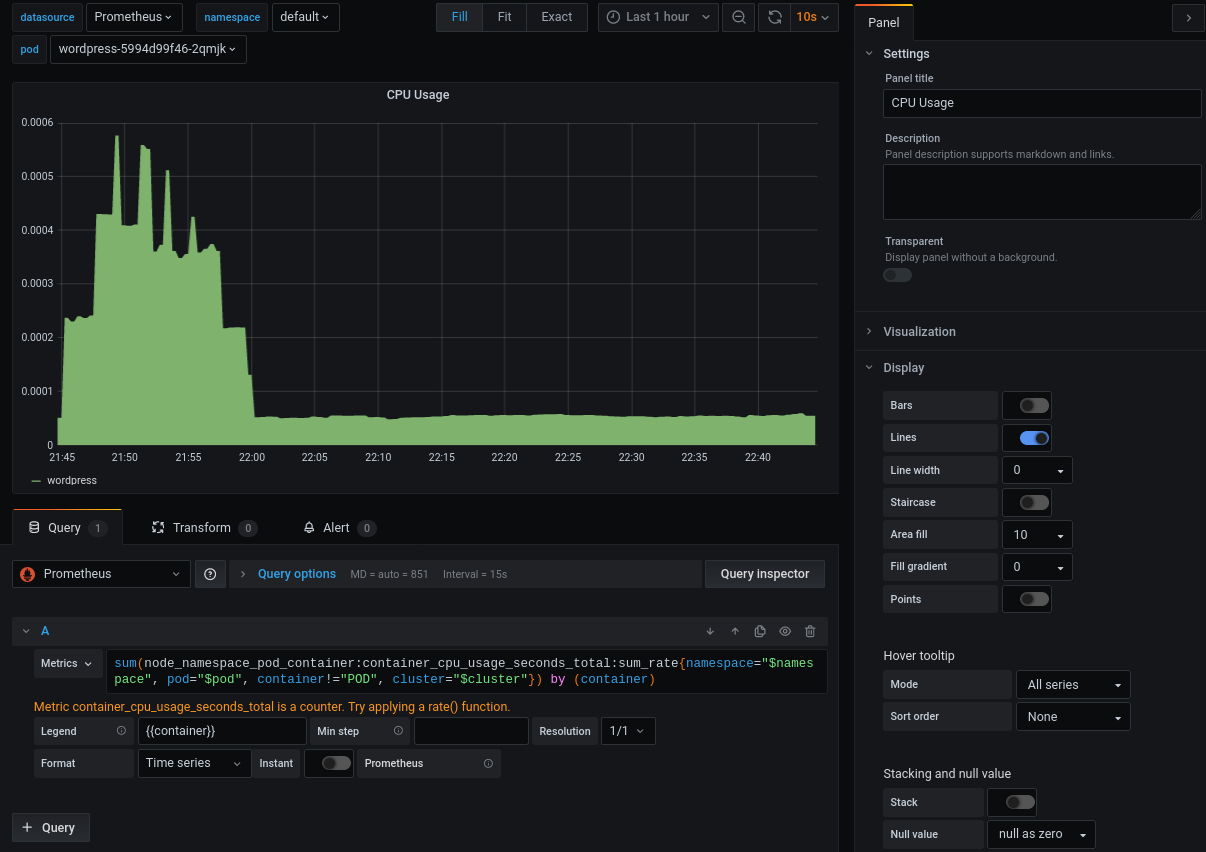
\includegraphics[width=1.1\textwidth]{img/panel1.png}
    \caption{Instellingen voor paneel 1 \autocite{Grafana}}
\end{figure}


Het tweede paneel dat gemaakt werd, was het paneel om het werkgeheugen gebruik te bekijken. Door een actie (installeren van een plugin/thema) uit te voeren op de WordPress site kon een verhoging van het werkgeheugen gebruik gezien worden in de meter. Bij ''settings'' kon de naam aangepast worden naar ''Memory Usage''. De afbeelding werd gebruikt om de nodige velden in te vullen.

\begin{figure}
    \centering
    \subfigure[]{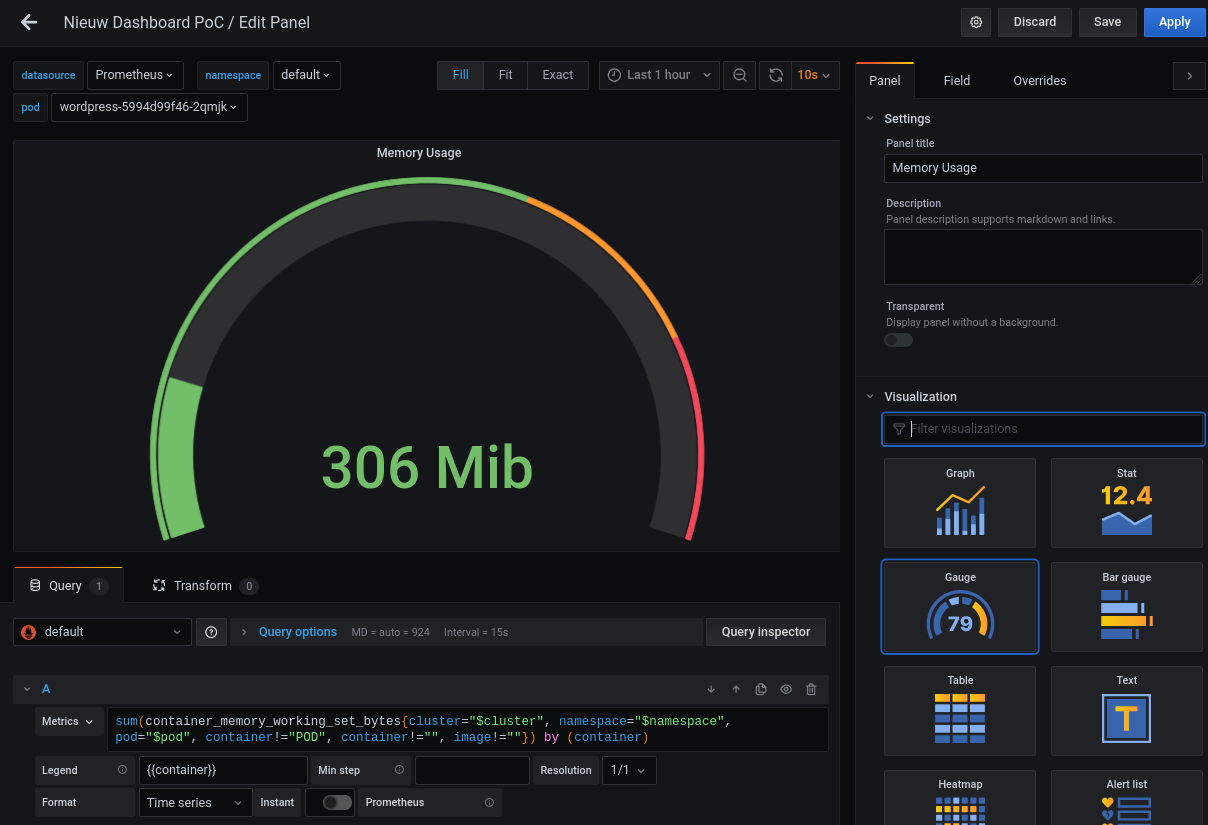
\includegraphics[width=1.1\textwidth]{img/panel2.png}}
    \subfigure[]{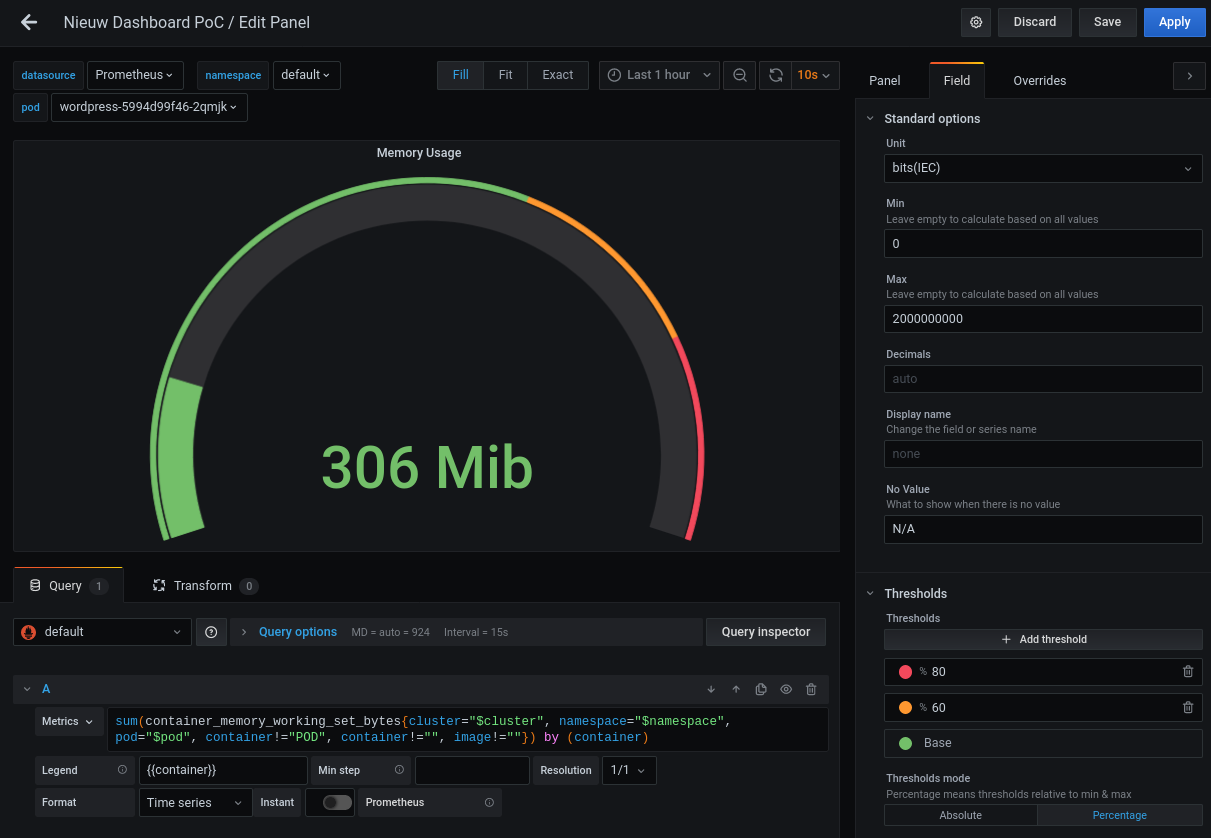
\includegraphics[width=1.1\textwidth]{img/panel3.png}} 
    \caption{Instellingen voor paneel 2 \autocite{Grafana}}
\end{figure}

\clearpage
Het derde paneel dat gemaakt werd, was het paneel om het netwerkverkeer te bekijken. Door een actie (downloaden van een plugin/thema) uit te voeren op de WordPress site kon een verhoging van het netwerkverkeer gezien worden in de grafiek. Bij ''settings'' kon de naam aangepast worden naar ''Network Usage''. De afbeelding werd gebruikt om de nodige velden in te vullen. ²

\begin{figure}[!h]
    \centering
        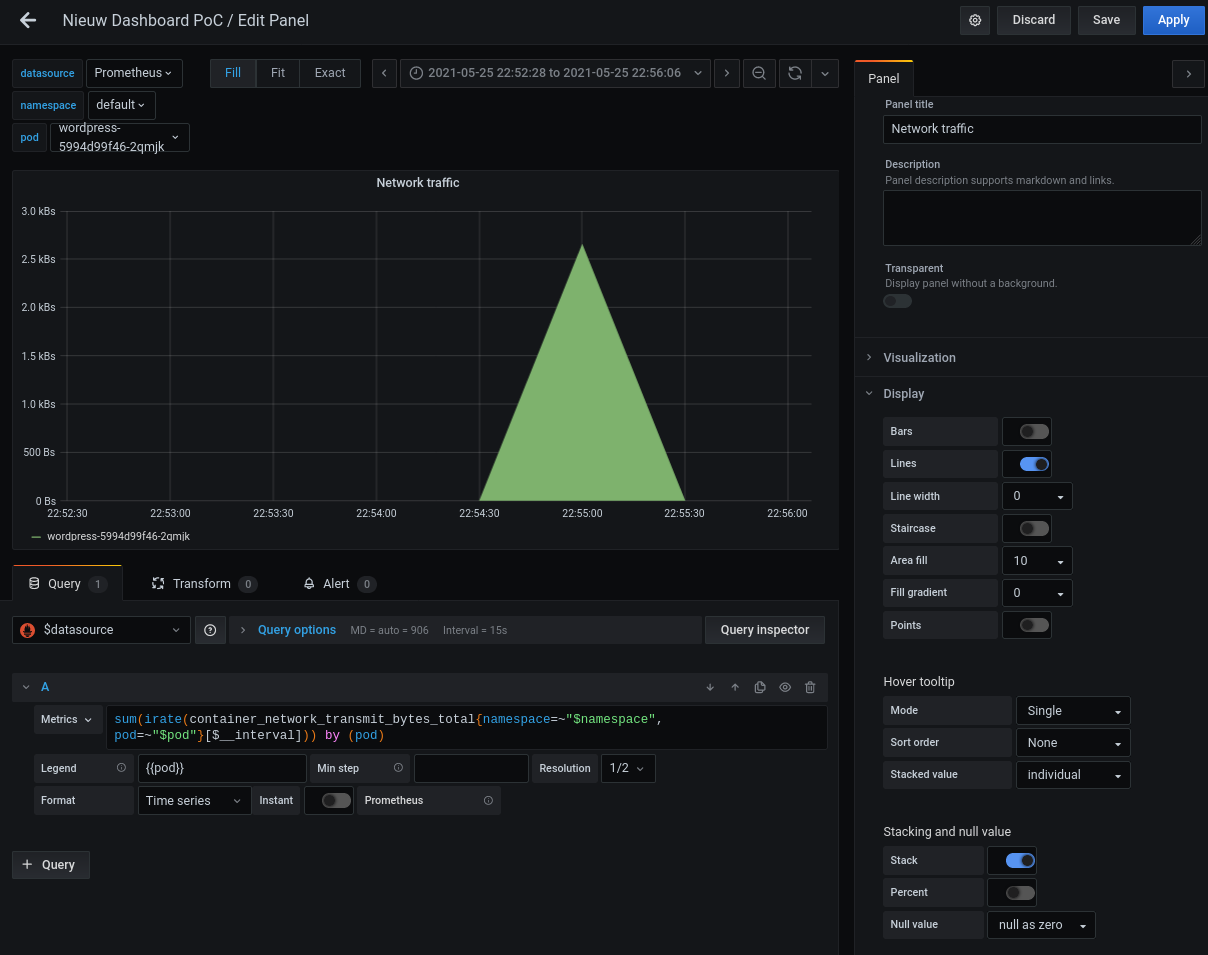
\includegraphics[width=1.1\textwidth]{img/panel4.png}
    \caption{Instellingen voor paneel 3 \autocite{Grafana}}
\end{figure}

\subsection{Stap 2.6: Grafana dashboard in werking}

Na het instellen van deze drie panelen, was er een dashboard beschikbaar waarbij de pod kon aangepast worden. Om te zien dat de grafieken en meters responsief waren op een mogelijke bewerking die in een pod plaatsvond, kon er gebruik gemaakt worden van \ref{sssec:Groeivancontainers} ''Groei van containers''. Hiervoor werd verwacht dat de pod op het dashboard ingesteld werd op een ''apache''pod waarop de groei van de containers zichtbaar was.
\clearpage

\subsection{Stap 2.7: Bereiken van de Prometheus webinterface}

Hoewel de webinterface van Grafana voorkeur had door de gebruiksvriendelijke manier, werd deze webinterface van Prometheus toch opgezet om de interface te kunnen bereiken. De interface was te bereiken via ''http://localhost:9090'' na het uitvoeren van het volgende commando.

\begin{lstlisting}[language=bash,caption={port forward prometheus}]
kubectl port-forward 
prometheus-prometheus-prometheus-oper-prometheus-0 9090
\end{lstlisting}

\subsection{Samenvatting}

Nu waren er drie webinterfaces die te bereiken waren voor de monitoring van de container omgeving, waarvan twee interfaces bijna volledig opgezet waren met een simpel commando door middel van ''Helm'' pakketten. 

\begin{itemize}
    \item Minikube Dashboard te bereiken via het ''MiniKube Dashboard'' commando
    \item Grafana Dashboard te bereiken via http://localhost:3000
    \item Prometheus Dashboard te bereiken via http://localhost:9090
\end{itemize}\clearpage

\section{Stap 3: Overlopen checklist}

Na het opstellen van de Proof-of-Concept werd een checklist overlopen met daarin de vooropgestelde vereisten voor een succesvolle Proof-of-Concept. Aan de hand van de checklist werd bepaald of de PoC goed genoeg was voor gebruik in het lessenpakket.

De checklist bestond uit de volgende punten:

\begin{itemize}
    \item De tool moet gratis zijn of de trial moet lang genoeg duren. 
    \item De tool moet voor een containeromgeving zijn.
    \item De volledige PoC moet lokaal geïnstalleerd zijn.
    \item De PoC moet mogelijk zijn op de laptop van de studenten die voldoet aan de opgelegde specificaties van HoGent.
    \item Via de Proof-Of-Concept moeten de functies van de monitoringtool goed genoeg zijn om de I/O metrics te analyseren.
    \item Aan de hand van één bestand kan de Proof-of-Concept opgezet worden zodat de studenten direct aan de slag kunnen met de monitoringtool.
    \item Installatie en configuratie moet van een gemiddeld niveau zijn.
    \item Opzetten van alerts.
    \item Het verzamelen en analyseren van logs. 
\end{itemize}

Uit de vorige checklijst kon het volgende geconcludeerd worden:

\begin{itemize}
    \item De tool was gratis. 
    \item De tool was geschikt voor een containeromgeving.
    \item De volledige PoC was lokaal geïnstalleerd.
    \item De PoC was mogelijk op de laptop van de studenten.
    \item Via de Proof-Of-Concept waren de functies van de monitoringtool goed genoeg om de I/O metrics te analyseren.
    \item Een OVA bestand was niet aanwezig om het makkelijk reproduceerbaar te maken maar werd wel door dit onderzoek ter beschikking gesteld.
    \item Installatie en configuratie waren van een gemiddeld niveau zijn.
    \item Opzetten van alerts was mogelijk maar niet uitgevoerd in dit bachelorproef.
    \item Het verzamelen en analyseren van logs was mogelijk  maar niet uitgevoerd in dit bachelorproef. 
\end{itemize}

